\section{Evaluation}
\label{sec:evaluation}

% Motivation for evaluation design
% May be more general aspects of aesthetics that our model captures, compared to random colorings or color compatibility only
We conducted an online judgement study to gain a better understanding of how coloring suggestions from our model compare to colorings from simpler models as well as colorings made by artists. We recruited 16 Computer Science graduate students (5 female) to participate in the study. All participants had normal color vision. To better simulate the exploratory situations in which our model would be used, we generate and present multiple coloring suggestions. Although different participants almost certainly have different aesthetic preferences, we should be able to see any general trends in the preferability of colorings generated by different methods. 

% Experiment Setup
\newcommand{\artistSource}{\emph{Artist}}
\newcommand{\modelSource}{\emph{Model}}
\newcommand{\compatSource}{\emph{Color Compatibility}}
\newcommand{\randomSource}{\emph{Random}}
We first generate a set of coloring suggestions from four different sources----\artistSource~colorings, our \modelSource, a \compatSource-only model using the measure by O'Donovan et. al.~\shortcite{ODonovan}, and \randomSource~colorings---to be compared in the study. Next, we select 15 different pattern templates that do not have strong semantic associations and are also outside of our training set. For each pattern template, we then generate 4 coloring suggestions per source. For the \artistSource~source, we randomly choose 4 colorings from the top 45 artist colorings on COLOURlovers. For our \modelSource, we sample colors using parallel tempering for 2000 iterations and choose the top 4 results using MMR with $\lambda = 0.5$. We similarly sample \compatSource-only colorings. Finally, for the \randomSource~source, we generate 4 random colorings.

The study interface presents participants with a randomized grid of all 16 coloring suggestions for a pattern template. Participants are asked to chose the 4 colorings they like the most and the 4 they like the least from the grid for this pattern template before moving on to the next template. Each participant responds to 5 pattern templates randomly drawn from the pool of 15 and presented in random order. In addition, one template is presented twice, to check for participant consistency.

Figure ~\ref{fig:study} shows the number of times suggestions from each source were chosen as a `Top 4' or `Bottom 4' pattern. When counting, we do not include suggestions from the replicated template. We use binomial regression to model the odds of each source being chosen as either a `Top 4' or `Bottom 4' suggestion. Tukey all-pair comparison tests show that all differences are significant ($p < 0.01$), except for the odds that an \artistSource~suggestion will be chosen as a `Bottom 4' suggestion versus a \modelSource~suggestion. \artistSource~patterns are selected most often as a `Top 4' pattern, with our \modelSource~patterns selected second most often. In addition, \modelSource~patterns are selected least as a `Bottom 4' pattern, along with \artistSource~patterns.

\begin{figure}[h!]
  \begin{center}
  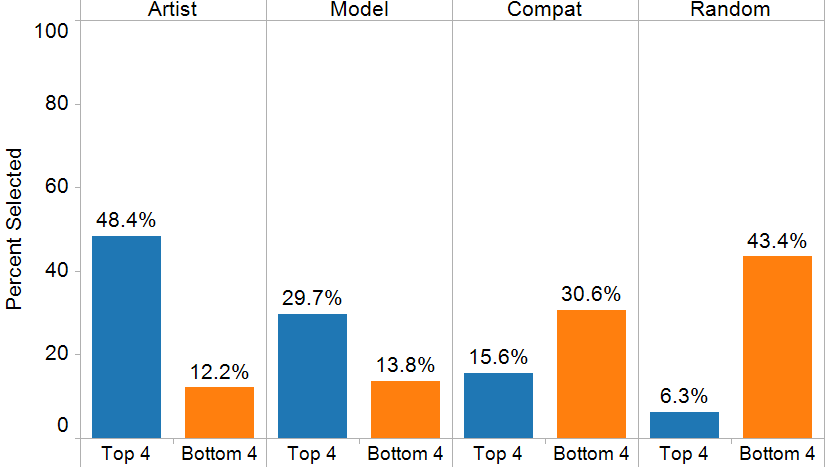
\includegraphics[width=\columnwidth]{figs/evaluation.png}
	\end{center}
\caption{The percentage of times that \artistSource-created, \modelSource-generated, \compatSource-only, and \randomSource~patterns were chosen by participants as one of their `Top 4' favorite or `Bottom 4' least favorite patterns in our online experiment.}

 \label{fig:study}
\end{figure}

The results of this study suggest that \modelSource-generated patterns have significantly higher quality than patterns generated by other automatic baseline approaches. They do not yet achieve the same quality as \artistSource-created patterns, but since our model functions as part of an interactive coloring workflow with a human in the loop, this result is acceptable. This research does not seek to replace human artists but rather to augment their abilities. The result that \modelSource~patterns are `disliked' as infrequently as \artistSource~patterns suggests that the \modelSource~patterns not chosen as favorites are likely good enough to serve as inspirational starting points for further creative work.